\documentclass{beamer}

% There are many different themes available for Beamer. A comprehensive
% list with examples is given here:
% http://deic.uab.es/~iblanes/beamer_gallery/index_by_theme.html
% You can uncomment the themes below if you would like to use a different
% one:
%\usetheme{AnnArbor}
%\usetheme{Antibes}
%\usetheme{Bergen}
%\usetheme{Berkeley}
%\usetheme{Berlin}
%\usetheme{Boadilla}
%\usetheme{boxes}
\usetheme{CambridgeUS}
%\usetheme{Copenhagen}
%\usetheme{Darmstadt}
%\usetheme{default}
%\usetheme{Frankfurt}
%\usetheme{Goettingen}
%\usetheme{Hannover}
%\usetheme{Ilmenau}
%\usetheme{JuanLesPins}
%\usetheme{Luebeck}
%\usetheme{Madrid}
%\usetheme{Malmoe}
%\usetheme{Marburg}
%\usetheme{Montpellier}
%\usetheme{PaloAlto}
%\usetheme{Pittsburgh}
%\usetheme{Rochester}
%\usetheme{Singapore}
%\usetheme{Szeged}
%\usetheme{Warsaw}

\title{LSINF1225 : Programmation orientée-objet et gestion de données}

% A subtitle is optional and this may be deleted
\subtitle{UCLove}

\author{D.~Schmitz\inst{1} \and C.~Deknop\inst{2} \and R.~Gielen\inst{3} \and A.~Deronne\inst{4} \and M.~Volon\inst{5}}
% - Give the names in the same order as the appear in the paper.
% - Use the \inst{?} command only if the authors have different
%   affiliation.

\institute[Université de Louvain-la-Neuve] % (optional, but mostly needed)
{
  \inst{1}%
  SINF11BA
  \and
  \inst{2}%
  SINF12BA
  \and
  \inst{3}%
  SINF12BA
  \and
  \inst{4}%
  SINF12BA
  \and
  \inst{5}%
  LING2MS/LA
  }
% - Use the \inst command only if there are several affiliations.
% - Keep it simple, no one is interested in your street address.

\date{UCLove, 2016}
% - Either use conference name or its abbreviation.
% - Not really informative to the audience, more for people (including
%   yourself) who are reading the slides online

\subject{Theoretical Computer Science}
% This is only inserted into the PDF information catalog. Can be left
% out. 

% If you have a file called "university-logo-filename.xxx", where xxx
% is a graphic format that can be processed by latex or pdflatex,
% resp., then you can add a logo as follows:

% \pgfdeclareimage[height=0.5cm]{university-logo}{university-logo-filename}
% \logo{\pgfuseimage{university-logo}}

% Delete this, if you do not want the table of contents to pop up at
% the beginning of each subsection:
\AtBeginSubsection[]
{
  \begin{frame}<beamer>{Outline}
    \tableofcontents[currentsection,currentsubsection]
  \end{frame}
}

% Let's get started
\begin{document}

\begin{frame}
  \titlepage
\end{frame}

\begin{frame}{Outline}
  \tableofcontents
  % You might wish to add the option [pausesections]
\end{frame}

% Section and subsections will appear in the presentation overview
% and table of contents.
\section{Introduction}

\subsection{UCLove...?}
\begin{frame}{UCLove...?}
\begin{block}{Application de rencontres}
	\begin{itemize}
		\item{
			accessibilit\'e (tablette/t\'el\'ephone Android)
		}
		\item{
			efficacit\'e, rapidit\'e (public h\'et\'erogene ou recherche cibl\'ee)
		}
		\item{
			\'ethique, confidentialit\'e (visibilit\'e des informations personnelles)
		}
	\end{itemize}
\end{block}
\begin{block}{Attentes "classiques"}
	\begin{itemize}
		\item{
			recherche de personnes (filtres disponibles)
		}
		\item{
			discussion instantan\'ee
		}
		\item{
			[organisation d'une rencontre r\'eelle]
		}
	\end{itemize}
\end{block}
\begin{block}{Pr\'esentation des fonctionnalit\'es de base}
\end{block}
\end{frame}

\begin{frame}
	\begin{itemize}
	
	\item{
	
	}
	\end{itemize}
\end{frame}
\section{Aperçu de l'application}

\subsection{Page d'acceuil}

\begin{frame}{First Slide Title}{Optional Subtitle}
  \begin{itemize}
  \item {
    Inscription
  }
  \item {
    Connexion
  }
  \end{itemize}
\end{frame}

\subsection{Menu principal}

% You can reveal the parts of a slide one at a time
% with the \pause command:
\begin{frame}{Second Slide Title}
  \begin{itemize}
  \item {
	Navigation
  }
  \end{itemize}
\end{frame}

\subsection{Profil}

\begin{frame}

	\begin{itemize}
	
	\item{
	Nom	
	}
	\item{
	Attributs physiques	
	}
	
	\item{
	Photo
	}
	\end{itemize}

\end{frame}

\subsection{Rencontre}
\begin{frame}
	\begin{itemize}
	\item{
	Profil d'un utilisateur
	}
	\item{
	Possibilité d'envoyer une requête ou de passer au profil suivant
	}
	\item{
	Filtre disponible
	}
	\end{itemize}
\end{frame}

\subsection{Requetes}
\begin{frame}
	\begin{itemize}
	\item{Demandes en attente}
	\item{
	Demande d'ajout d'autres utilisateurs
	}
	
	\end{itemize}
\end{frame}



\subsection{Amis}
\begin{frame}
	\begin{itemize}
	\item{
	Liste d'utilisateurs ajoutés
    
	}
	\item{Utilisateur favoris}
	
	\end{itemize}
\end{frame}

\subsection{Options}
\begin{frame}
\begin{itemize}
    \item{Choix de la langue}
    \item{Deconnexion}
    
\end{itemize}
\end{frame}

\subsection{Disponibilités}
\begin{frame}
  \begin{itemize}
      \item{}
  \end{itemize}
\end{frame}


\section{Aspects techniques}

\subsection{Base de données}

\begin{frame}
  \begin{figure} 
  	\centering 
  	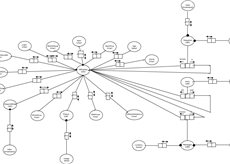
\includegraphics[scale=0.9]{pictures/schema_database.jpg} 
  	\caption{Schéma de la base de donnée} 
  	\label{fig:my_label} 
  \end{figure}
\end{frame}



\subsection{Implémentation}
\begin{frame}
  \begin{figure} 
	\centering 
	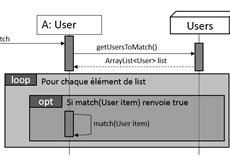
\includegraphics[scale=0.8]{pictures/sequence_match.jpg} 
	\caption{Diagramme de séquence pour l'activity Match} 
	\label{fig:my_label} 
  \end{figure}
\end{frame}

\section{Conclusion}

\subsection{Bilan}



\subsection{Perspectives}
\begin{frame}
  \begin{itemize}
      \item{Disponibiltés}
      \item{Confidentialité}
      \item{Interface graphique originale}
      \item{Base de données sur un serveur distant}
  \end{itemize}
\end{frame}

% Placing a * after \section means it will not show in the
% outline or table of contents.
\section*{Summary}

\begin{frame}{Summary}
  \begin{itemize}
  \item
    The \alert{first main message} of your talk in one or two lines.
  \item
    The \alert{second main message} of your talk in one or two lines.
  \item
    Perhaps a \alert{third message}, but not more than that.
  \end{itemize}
  
  \begin{itemize}
  \item
    Outlook
    \begin{itemize}
    \item
      Something you haven't solved.
    \item
      Something else you haven't solved.
    \end{itemize}
  \end{itemize}
\end{frame}



% All of the following is optional and typically not needed. 
\appendix
\section<presentation>*{\appendixname}
\subsection<presentation>*{For Further Reading}

\begin{frame}[allowframebreaks]
  \frametitle<presentation>{For Further Reading}
    
  \begin{thebibliography}{10}
    
  \beamertemplatebookbibitems
  % Start with overview books.

  \bibitem{Author1990}
    A.~Author.
    \newblock {\em Handbook of Everything}.
    \newblock Some Press, 1990.
 
    
  \beamertemplatearticlebibitems
  % Followed by interesting articles. Keep the list short. 

  \bibitem{Someone2000}
    S.~Someone.
    \newblock On this and that.
    \newblock {\em Journal of This and That}, 2(1):50--100,
    2000.
  \end{thebibliography}
\end{frame}

\end{document}


